% TEMPLATE for Usenix papers, specifically to meet requirements of
%  USENIX '05
% originally a template for producing IEEE-format articles using LaTeX.
%   written by Matthew Ward, CS Department, Worcester Polytechnic Institute.
% adapted by David Beazley for his excellent SWIG paper in Proceedings,
%   Tcl 96
% turned into a smartass generic template by De Clarke, with thanks to
%   both the above pioneers
% use at your own risk.  Complaints to /dev/null.
% make it two column with no page numbering, default is 10 point

% Munged by Fred Douglis <douglis@research.att.com> 10/97 to separate
% the .sty file from the LaTeX source template, so that people can
% more easily include the .sty file into an existing document.  Also
% changed to more closely follow the style guidelines as represented
% by the Word sample file. 

\documentclass[twocolumn,10pt]{article}
\usepackage[a4paper, top=1.0in, bottom=1.0in, left=0.8in, right=0.8in]{geometry}
\usepackage{endnotes}
\usepackage{graphicx}
\usepackage{listings}
\usepackage{xcolor}
\graphicspath{{figure/}}
\usepackage{listings} 
\usepackage{biblatex}
\bibliography{ref}

\begin{document}

%don't want date printed
\date{}

%make title bold and 14 pt font (Latex default is non-bold, 16 pt)
\title{\bf Grouper: A Group Finance Manager Using Secret Sharing and Data Synchronization on Mobile devices}

%\author{Department of Computer Science, Graduate School of Systems and Information Engineering 
%	\\Meng Li 201620728  
%	\\Supervisor Yasushi Shinjo
%	\\November 17th, 2016}

\maketitle

\section{Introduction}
The conventional applications are based on a client-server mode, which requires a central server for storing shared data. That means the users of the web applications must fully trust central servers and their application providers. Once a server is attacked by hackers, user information may be revealed because data is stored on only one server with cleartext. Finally, users may lose their data when service providers shut down their services.

Thus, we are going to implement a group finance manager application: Grouper, which is not relied on central servers, that means user data cannot be cracked easily and its service can be recovered after shutting down the old service. Recently, Most popular way is using P2P(Peer to Peer) to transfer user data between devices. However, there is a obvious problem in such a no-server proposal. Synchronization can only be finished in condition that two devices is online in a same time. Another problem is that the number of P2P connections will be increased fast with the increasing of group scale because each device can create a connection to all of the other devices. 

To address this problem without using P2P, we are considering to use multiple servers to build an untrusted server group. Data will divided to several pieces and uploaded to diverse servers. Each server can only save a piece of data temporarily,which means this piece will be deleted after a period time we specified. Those two rules explained above can ensure that user data cannot be cracked easily. In fact, we can regard the server group as a bridge between devices of group members. In addition, all devices of group members have saved a complete data set, data can be recovered theoretically even the server group breaks down. By this way, we think such a method can satisfy the requirements for an application which is running on untrusted server group, and not relied on central servers.

\section{Related Work}

DepSky\cite{bessani2013depsky} is a system that storage encrypted data on servers and run application logic on the client-side\cite{wang2016sieve}. DepSky provide a storage service that improves the availability and confidentiality provided by commercial storage cloud services. \emph{Cloud-of-Clouds} is the core concept in DepSky. It represents that DepSky is a virtual storage cloud, which is accessed by its users by invoking operations in several individual severs. DepSky saves encrypted data in commercial storage cloud services and do application logic in individual servers. In Grouper,  server group undertake responsibility of temporarily data storage and message delivery with server-side computation. Thus, Grouper cannot only use commercial storage cloud services.

Mylar\cite{popa2014building} stores sensitive data encrypted on the server, and decrypts that data only in users’ browsers. Like Grouper, application in Mylar can control how user data is shared\cite{wang2016sieve}; unlike Grouper, Mylar build its system on a browser with browser extension while Grouper use mobile devices as client.

Of course, there are many applications or frameworks synchronize with untrusted network and servers. Compared to them, Grouper use secret sharing and temporary data storage with untrusted server group to protect user data from malicious attacking.
\section{Methodology}

We consider that implementing such a distributed application Grouper on mobile devices is easier than PC, due to the reason that mobile devices can access to Internet by cellular network everywhere and every time. For this reason, we implement Grouper on iOS devices. 

\subsection{Data Sync with Untrusted Server Group}

We implement Grouper based on data synchronization by multiple servers rather than one central server. The main difference between our proposal and the traditional way using central server is that Grouper is not relying on server. There are three principles in our proposal. 

The first is data transfer by server, not save on server. Most current popular B/S modal application storage user data on several central servers, user data will not be deleted unless user delete his account. Grouper use server as a bridge for transferring data. Considering a group including three members Alice, Bob and Carol. Alice created a new record in her device, this record will be upload to server group, and will not exist after Bob and Carol synchronized it from server group. In other words, server group storage a record until it is be synchronized by all group members.

The second is server save data uploaded from mobile devices temporarily. We define a period of time in which data can be saved in a server. In this paper, we set this period to 1 hour for our example situations, that means the record Alice uploaded to server group can only be saved for 1 hour. After 1 hour since uploaded, this record will be deleted. Alice is required to resend this record to server group until all of other members has synchronized successfully. It is obvious that this period of time should be long while more members attend the group. However, the longer saving period means the higher risk of data reveal. The most suitable period is influenced by the number of group members, security requirement, user expectations and so on. 

The third is server does not know the content of data. Only by saving data temporarily cannot ensure data security, because server knows the cleartext of data in this temporary period. For this problem, developers encrypt data before uploading to servers, which need a private key to decrypt data in other devices. In order to distribute the private key, users should share by themselves. In this paper, we are going to use secret sharing, which can create a number of shares and distributing them to a set of participants\cite{smith2013layered}, to share data between user devices and server group.

\begin{figure}[t]
\centering
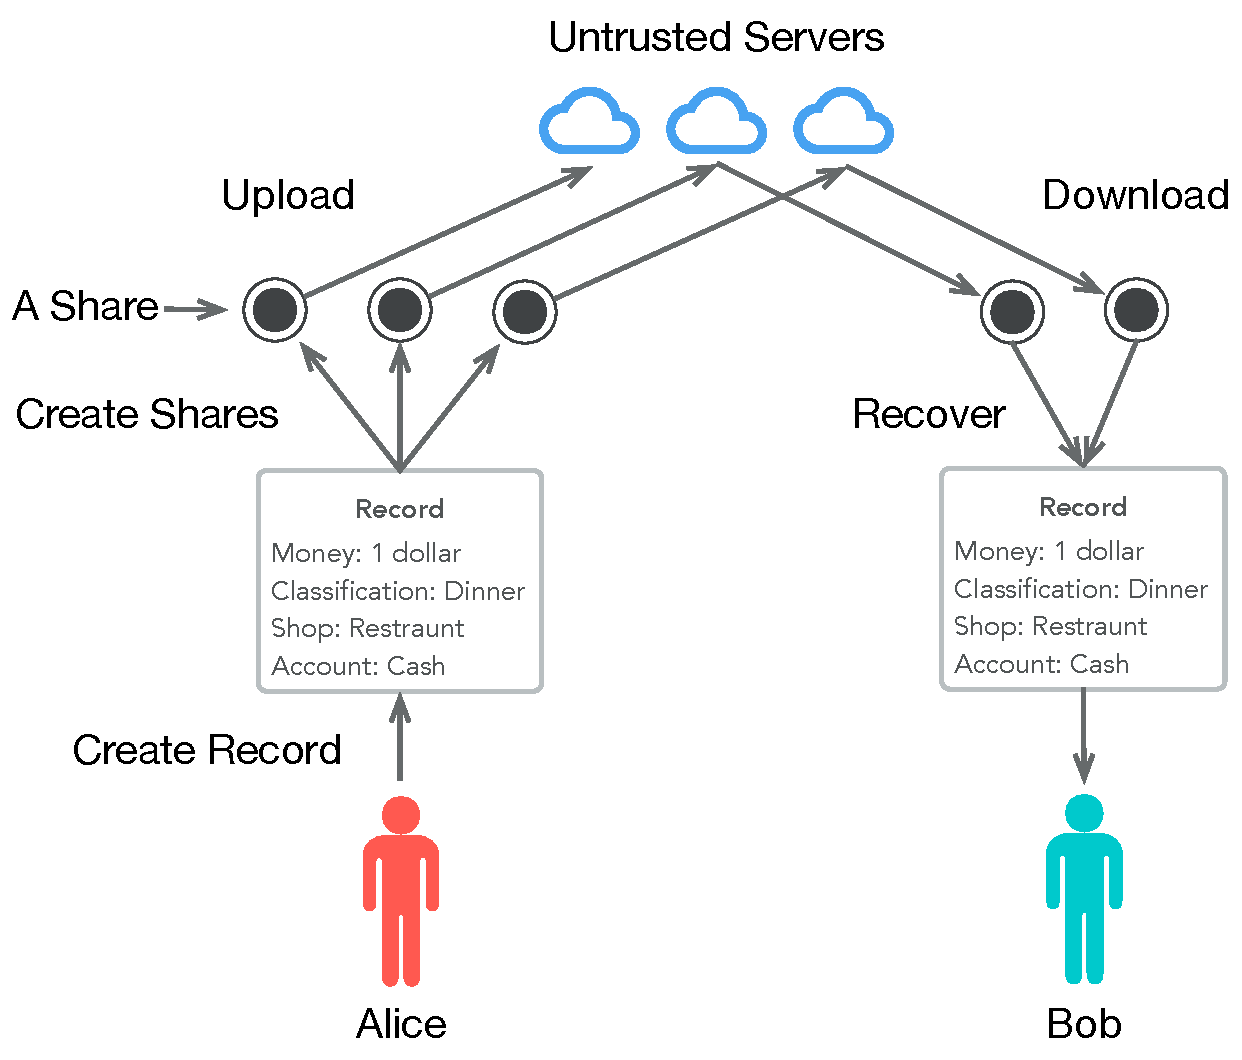
\includegraphics[scale=0.4]{sync_flow}
\caption{Flow of Synchronization}
\end{figure}
Based on the three core principles introduced above, our synchronization flow can be described as figure 1. At first, Alice create a record including money, classification, shop and account. Grouper create a number of shares by secret sharing and upload those shares to server group. When Bob is online, Grouper in Bob's device will download shares from server group and recover the new record uploaded by Alice. In our situation, Grouper can recover the record after getting more than two shares. In this process, each server is separated from other server, and cannot access to other server, which means user data cannot be recovered unless you have permission access to more than two server. In our proposal, only group members have permission to access server group.


\subsection{Shamir's Secret Sharing}
Secret sharing which can create a numbers of shares, plays an indispensable role in protecting user data from getting lost, destroyed, or into wrong hands. In this paper, we are going to use Shamir's secret sharing, a form of secret sharing proposed by Shamir and Blakley independently. In secret sharing scheme, a dealer securely shares a secret with a group of participants, by generating $n$ shares using a cryptographic function\cite{smith2013layered}. At least $k$ or more participants can reconstruct the secret, but $k-1$ or fewer participants can obtain nothing about the secret\cite{pang2005new}. We describe this scheme as a function $f(k, n)$, n is the number of all shares, and k is the threshold to combine shares. A popular technique to implement threshold schemes uses polynomial interpolation ("Lagrange interpolation"). This method was invented by Shamir in 1979. Thus, we call it Shamir's Secret Sharing.

There are many implementations of Shamir's secret sharing by different programming languages. For developing an iOS app by Objective-C, we need an implementation without limitation of length, which supports Objective-C language and UTF-8 character set. c-SSS\cite{c-sss} is an implementation in original C code of Shamir's Secret Sharing by Fletcher T. Penney. c-SSS provide two main functions for generate shares and reconstructing them. Function \emph{generate} can generate $n$ shares by the string text with the threshold $k$. Function \emph{extract} can recreate the text string after accessing to more than $k$ shares.

\subsection{Synchronize Completely}
There is no doubt that Grouper should provide a reliable synchronization service. For Alice, once she created a new record in her device, all of other members in a group should synchronize this record, even if this record may be deleted by server group after 1 hour. We call this problem \emph{Synchronize Completely}.

\begin{figure}[t]
\centering
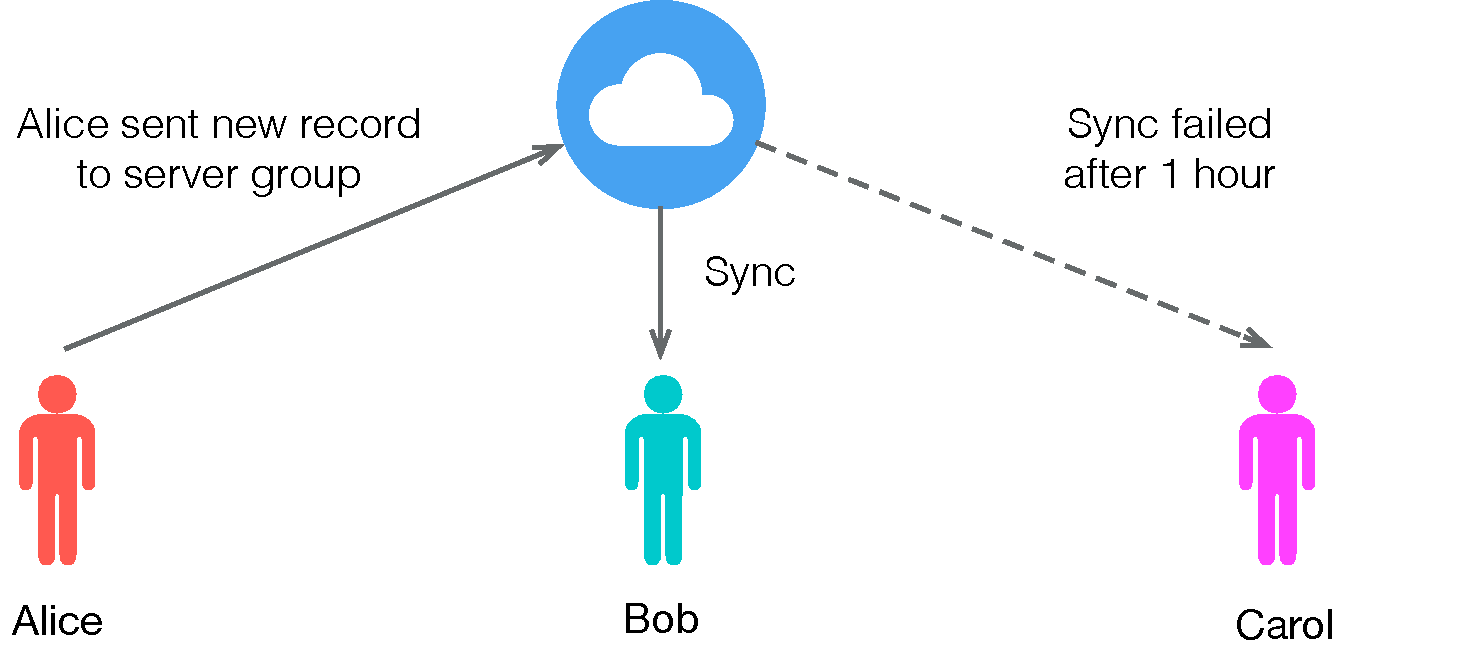
\includegraphics[scale=0.4]{sync_completely}
\caption{Sync Completely}
\end{figure}

Figure 2 described the situation data cannot be synchronized completely. Alice sent a new record to server group in 10:00 AM and Bob synchronized it successfully before 11:00 AM. Carol forgot to synchronize this record before 11:00 AM. She cannot synchronize after 11:00 AM because server group has delete the record in 11:00 AM. To solve this problem, Alice is required to resend her new record until Carol synchronize it successfully. However, by what way can Alice get the information that all of other members in her group have synchronized. In other words, it is an unreasonable requests for Alice to resend her record indefinitely. It is necessary for us to find a efficient way for notifying Alice that all members have synchronized successfully.

We are going to design a counter in clients as the solution to \emph{Sync Completely} problem. Intuitively, this counter which can calculate the number of times other clients synchronized, works on the sender to decide resending record or not. The condition that sender device need not resend record can be described as equation 1.
\begin{equation}
\sum_{i=1}^{n}s_{i}=(m-1)\cdot k
\end{equation}

In equation 1, we suppose that there are $n$ servers in our server group , they are server 1, server 2,..., server $n$. We can also look at $n$ from a different perspective, it is first parameter, the number of all shares, in the scheme $f(k, n)$ of Shamir's secret sharing. Each server saves a share, so $n$ servers saves $n$ shares. Each server should know how many times the share has been downloaded by clients. Thus, we use $s_i$ to represent the number of times in server $i$. The sum of $s_i$ is calculated in sender client. In the left of equation 1, $m$ represents the number of group members, and $k$ is the threshold in scheme $f(k, n)$. Obviously, a client can reconstruct data after getting $k$ shares. If $m-1$ clients have reconstructed data, $(m-1)\cdot k$ shares is downloaded. That means clients except sender has synchronized successfully, so sender need not resend.

To implement such a counter, restriction about security and connection should be considered. On the one hand, servers cannot communicate with each other. Actually, one server of the group does not know the others exist in the group. On the other hand, clients cannot communicate with each other. Clients do know IP address or domain name of other device, so that they cannot send message with P2P connections. We decide to design a sync table described as figure 3, which is running on both servers and client to statistic sync times. Sync tables dominates all the synchronization activity in Grouper. Physical id, content, and count of sync times are main column in sync table. Physical id is an unique identifier created by SQLite database in client, it is same as those in servers. Content in client saves the JSON string converted by new record object. In server, it saves one of the shares generated by secret sharing scheme. Count, the core column in sync table, saves the content sync times in server. In client, count saves the sum of all counts from server. Of course, physical id of count in client and counts in servers are same. Suppose the secret sharing scheme is $f(2, 3)$, and only Bob have synchronized Alice's new record within prescribed time-limit. In figure 3, the column corresponding to Alice's new record, whose id is 1, is equals to those columns whose ids are 1 in server 1 and server 2. This is to say Bob downloaded two shares from server 1 and server 2. Client of Alice will know that by HTTP response from server 1 and server 2 when it resend data. It will send for one more time, because it's count is 2, which is less than 4, the threshold Alice need not resend.

\begin{figure}[t]
\centering
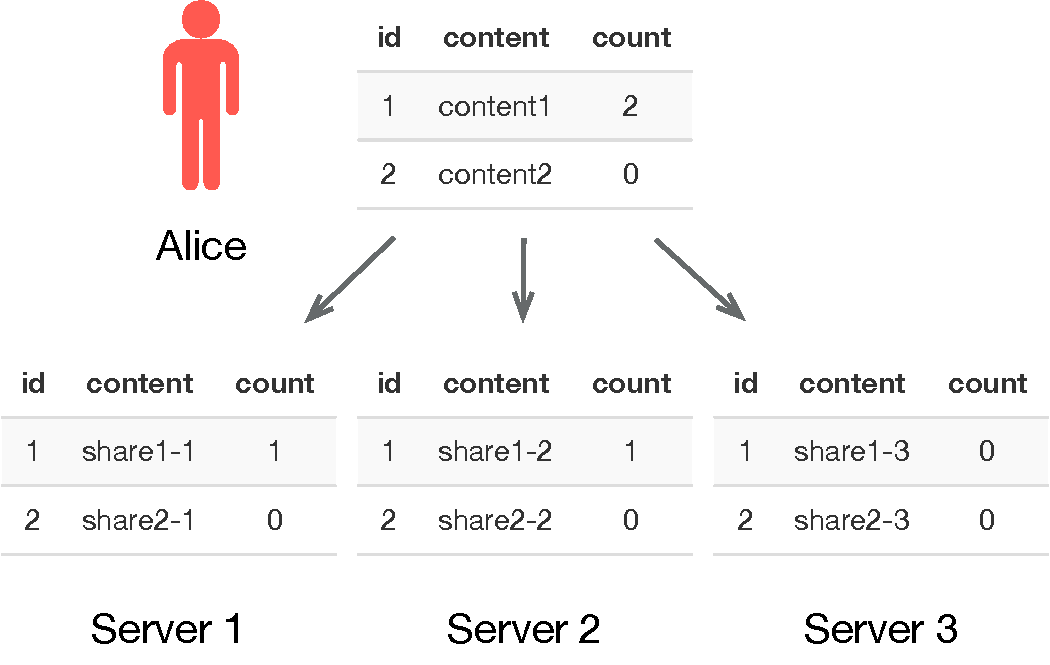
\includegraphics[scale=0.4]{sync_table}
\caption{Sync Table}
\end{figure}

\section{Architecture}
Grouper includes an iOS app for clients and a web service in server group.

\subsection{Architecture in Client}
In Methodology, we have introduced how to sharing a string with other deices via untrusted server group. In this paragraph, let us talk about persistent store and data synchronization before architecture. With untrusted server group, Grouper have to storage all data on mobile devices with an object-oriented way. Grouper use Core Data\cite{coredata}, a native iOS framework to manage the model layer objects, which provides generalized and automated solutions to common tasks associated with object life cycle and object graph management, including persistence, to storage and operate data as object. Sync\cite{sync} by Elvis Nuñez, a modern swift JSON synchronization framework to Core Data, can help we complete data synchronization easily in Grouper by parsing a JSON response and getting it into Core Data. With Sync based on Core Date, we can concentrate on sharing with untrusted server group rather than data storage and synchronization.

c-SSS by Fletcher T. Penney can generate shares from a JSON string saved on sync table. Grouper develop with Objective-C language, which is compatible with original C code. Grouper will generate shares and send them by REST API to server group until this record need not to resend. Response of REST API contains the count of sync times in server group, for calculating the sum and deciding wether resend or not.

\begin{figure}[t]
\centering
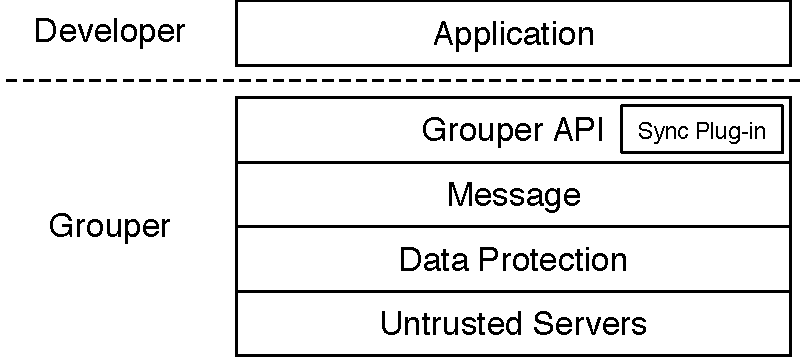
\includegraphics[scale=0.4]{architecture}
\caption{Architecture}
\end{figure}

\subsection{Necessity of Having a Web Service}
Many applications with synchronization is based on cloud services like Amazon S3, Google Cloud or iCloud. Here, Grouper does not synchronized via such cloud services for following reasons.
\begin{itemize}
\setlength{\itemsep}{1pt}
\setlength{\parskip}{0pt}
\setlength{\parsep}{0pt}
    \item Object-oriented: It is better for web service of Grouper to access data by object, while cloud service provide a way by document. 
    \item Controllability: It is more convenient to control when a new row in database should be added, deleted or modified by web service of ourself. 
    \item Computing in Server: Web service need collaborate with client to statistic sync times, which requires to calculate sync times in server.
\end{itemize}

\section{Future Work}

An application running in client has been developed now. In future, we are going to develop a web service running on untrusted server group to manage data temporary storage and provide REST API for mobile devices. This web service developed by Java EE should be install by group owner, in order that nobody except the group owner know all the IP address of servers. Thus, security of Grouper can be guaranteed.

\section{Conclusion}

This paper introduced Grouper, a group finance manager, using secret sharing and data synchronization on mobile devices. Grouper is synchronized by untrusted server group, each server of which does not know existence of others. Each server only saves one of the shares generated by secret sharing temporarily, to ensure that user data cannot be cracked easily.

{\tiny
\printbibliography
}

\end{document}

























